\subsubsection{Resultados}
\par Se presentan a continuaci\'on los resultados de la experimentaci\'on
    del algoritmo exacto para \emph{CMF}. La experimentaci\'on se realiz\'o
    con las instancias ya generadas (seg\'un se explica en \emph{\nameref{notas_preliminares},
    \nameref{notas:datasets}} y \emph{\nameref{notas:experimentacion}}).

\par Para recordar, se cuentan con 10 instancias aleatorias de cada tama\~no,
    las cuales fueron resueltas 5 veces cada una y nos quedamos con el menor tiempo
    requerido de esas 5 ejecuciones. Por \'ultimo, tomamos el promedio de este tiempo
    requerido calculado entre las instancias del mismo tama\~no (10, como se ha
    dicho).

\bigskip

\par Para comenzar, consideramos primero una familia de grafos completos, para
    los cuales se espera obtener un resultado mucho mejor que la complejidad
    exponencial del peor caso, por lo detallado en \emph{\nameref{backtracking:poda:grafo_completo}}

\begin{figure}[H]
    \centering
    \fontsize{8}{10}\selectfont
    \resizebox{0.8\textwidth}{!}{% GNUPLOT: LaTeX picture with Postscript
\begingroup
  \makeatletter
  \providecommand\color[2][]{%
    \GenericError{(gnuplot) \space\space\space\@spaces}{%
      Package color not loaded in conjunction with
      terminal option `colourtext'%
    }{See the gnuplot documentation for explanation.%
    }{Either use 'blacktext' in gnuplot or load the package
      color.sty in LaTeX.}%
    \renewcommand\color[2][]{}%
  }%
  \providecommand\includegraphics[2][]{%
    \GenericError{(gnuplot) \space\space\space\@spaces}{%
      Package graphicx or graphics not loaded%
    }{See the gnuplot documentation for explanation.%
    }{The gnuplot epslatex terminal needs graphicx.sty or graphics.sty.}%
    \renewcommand\includegraphics[2][]{}%
  }%
  \providecommand\rotatebox[2]{#2}%
  \@ifundefined{ifGPcolor}{%
    \newif\ifGPcolor
    \GPcolortrue
  }{}%
  \@ifundefined{ifGPblacktext}{%
    \newif\ifGPblacktext
    \GPblacktexttrue
  }{}%
  % define a \g@addto@macro without @ in the name:
  \let\gplgaddtomacro\g@addto@macro
  % define empty templates for all commands taking text:
  \gdef\gplbacktext{}%
  \gdef\gplfronttext{}%
  \makeatother
  \ifGPblacktext
    % no textcolor at all
    \def\colorrgb#1{}%
    \def\colorgray#1{}%
  \else
    % gray or color?
    \ifGPcolor
      \def\colorrgb#1{\color[rgb]{#1}}%
      \def\colorgray#1{\color[gray]{#1}}%
      \expandafter\def\csname LTw\endcsname{\color{white}}%
      \expandafter\def\csname LTb\endcsname{\color{black}}%
      \expandafter\def\csname LTa\endcsname{\color{black}}%
      \expandafter\def\csname LT0\endcsname{\color[rgb]{1,0,0}}%
      \expandafter\def\csname LT1\endcsname{\color[rgb]{0,1,0}}%
      \expandafter\def\csname LT2\endcsname{\color[rgb]{0,0,1}}%
      \expandafter\def\csname LT3\endcsname{\color[rgb]{1,0,1}}%
      \expandafter\def\csname LT4\endcsname{\color[rgb]{0,1,1}}%
      \expandafter\def\csname LT5\endcsname{\color[rgb]{1,1,0}}%
      \expandafter\def\csname LT6\endcsname{\color[rgb]{0,0,0}}%
      \expandafter\def\csname LT7\endcsname{\color[rgb]{1,0.3,0}}%
      \expandafter\def\csname LT8\endcsname{\color[rgb]{0.5,0.5,0.5}}%
    \else
      % gray
      \def\colorrgb#1{\color{black}}%
      \def\colorgray#1{\color[gray]{#1}}%
      \expandafter\def\csname LTw\endcsname{\color{white}}%
      \expandafter\def\csname LTb\endcsname{\color{black}}%
      \expandafter\def\csname LTa\endcsname{\color{black}}%
      \expandafter\def\csname LT0\endcsname{\color{black}}%
      \expandafter\def\csname LT1\endcsname{\color{black}}%
      \expandafter\def\csname LT2\endcsname{\color{black}}%
      \expandafter\def\csname LT3\endcsname{\color{black}}%
      \expandafter\def\csname LT4\endcsname{\color{black}}%
      \expandafter\def\csname LT5\endcsname{\color{black}}%
      \expandafter\def\csname LT6\endcsname{\color{black}}%
      \expandafter\def\csname LT7\endcsname{\color{black}}%
      \expandafter\def\csname LT8\endcsname{\color{black}}%
    \fi
  \fi
  \setlength{\unitlength}{0.0500bp}%
  \begin{picture}(7200.00,5040.00)%
    \gplgaddtomacro\gplbacktext{%
      \csname LTb\endcsname%
      \put(1562,924){\makebox(0,0)[r]{\strut{} 0}}%
      \csname LTb\endcsname%
      \put(1562,1500){\makebox(0,0)[r]{\strut{} 100000}}%
      \csname LTb\endcsname%
      \put(1562,2076){\makebox(0,0)[r]{\strut{} 200000}}%
      \csname LTb\endcsname%
      \put(1562,2652){\makebox(0,0)[r]{\strut{} 300000}}%
      \csname LTb\endcsname%
      \put(1562,3227){\makebox(0,0)[r]{\strut{} 400000}}%
      \csname LTb\endcsname%
      \put(1562,3803){\makebox(0,0)[r]{\strut{} 500000}}%
      \csname LTb\endcsname%
      \put(1562,4379){\makebox(0,0)[r]{\strut{} 600000}}%
      \csname LTb\endcsname%
      \put(1694,704){\makebox(0,0){\strut{} 0}}%
      \csname LTb\endcsname%
      \put(2546,704){\makebox(0,0){\strut{} 500}}%
      \csname LTb\endcsname%
      \put(3397,704){\makebox(0,0){\strut{} 1000}}%
      \csname LTb\endcsname%
      \put(4249,704){\makebox(0,0){\strut{} 1500}}%
      \csname LTb\endcsname%
      \put(5100,704){\makebox(0,0){\strut{} 2000}}%
      \csname LTb\endcsname%
      \put(5952,704){\makebox(0,0){\strut{} 2500}}%
      \csname LTb\endcsname%
      \put(6803,704){\makebox(0,0){\strut{} 3000}}%
      \put(176,2651){\rotatebox{-270}{\makebox(0,0){\strut{}Tiempo (nanosegundos)}}}%
      \put(396,2651){\rotatebox{-270}{\makebox(0,0){\strut{}(Escala Lineal)}}}%
      \put(4248,374){\makebox(0,0){\strut{}Cantidad de Nodos}}%
      \put(4248,154){\makebox(0,0){\strut{}(Escala Lineal)}}%
      \put(4248,4709){\makebox(0,0){\strut{}Tiempo de ejecución conforme aumenta la cantidad de nodos}}%
    }%
    \gplgaddtomacro\gplfronttext{%
      \csname LTb\endcsname%
      \put(5816,1317){\makebox(0,0)[r]{\strut{}Grafos Completos}}%
      \csname LTb\endcsname%
      \put(5816,1097){\makebox(0,0)[r]{\strut{}Cota teórica lineal $\mathcal O(n)$}}%
    }%
    \gplbacktext
    \put(0,0){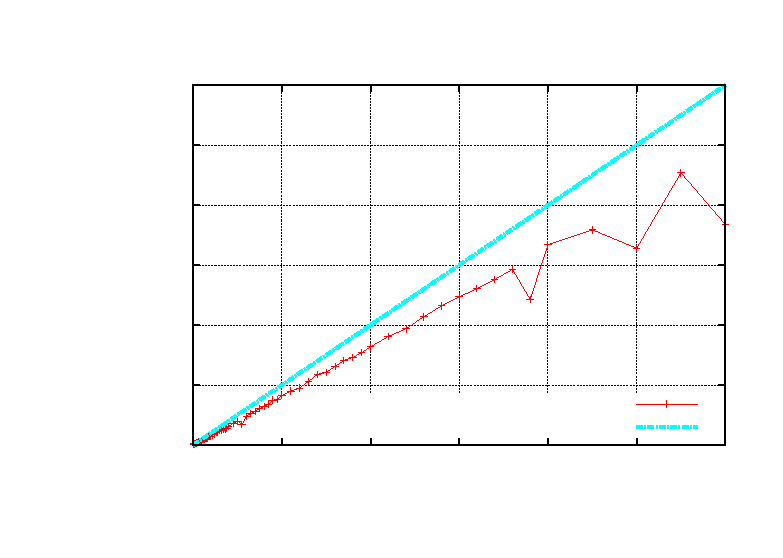
\includegraphics{ej2_nodos_completos}}%
    \gplfronttext
  \end{picture}%
\endgroup
}
    \caption{Algoritmo exacto seg\'un la densidad de los grafos}
\end{figure}

\bigskip

\par Siguiendo con la experimentaci\'on, ahora detallamos los resultados para las
    familias definidas seg\'un su densidad.

\begin{figure}[H]
    \centering
    \fontsize{8}{10}\selectfont
    \resizebox{1.0\textwidth}{!}{% GNUPLOT: LaTeX picture with Postscript
\begingroup
  \makeatletter
  \providecommand\color[2][]{%
    \GenericError{(gnuplot) \space\space\space\@spaces}{%
      Package color not loaded in conjunction with
      terminal option `colourtext'%
    }{See the gnuplot documentation for explanation.%
    }{Either use 'blacktext' in gnuplot or load the package
      color.sty in LaTeX.}%
    \renewcommand\color[2][]{}%
  }%
  \providecommand\includegraphics[2][]{%
    \GenericError{(gnuplot) \space\space\space\@spaces}{%
      Package graphicx or graphics not loaded%
    }{See the gnuplot documentation for explanation.%
    }{The gnuplot epslatex terminal needs graphicx.sty or graphics.sty.}%
    \renewcommand\includegraphics[2][]{}%
  }%
  \providecommand\rotatebox[2]{#2}%
  \@ifundefined{ifGPcolor}{%
    \newif\ifGPcolor
    \GPcolortrue
  }{}%
  \@ifundefined{ifGPblacktext}{%
    \newif\ifGPblacktext
    \GPblacktexttrue
  }{}%
  % define a \g@addto@macro without @ in the name:
  \let\gplgaddtomacro\g@addto@macro
  % define empty templates for all commands taking text:
  \gdef\gplbacktext{}%
  \gdef\gplfronttext{}%
  \makeatother
  \ifGPblacktext
    % no textcolor at all
    \def\colorrgb#1{}%
    \def\colorgray#1{}%
  \else
    % gray or color?
    \ifGPcolor
      \def\colorrgb#1{\color[rgb]{#1}}%
      \def\colorgray#1{\color[gray]{#1}}%
      \expandafter\def\csname LTw\endcsname{\color{white}}%
      \expandafter\def\csname LTb\endcsname{\color{black}}%
      \expandafter\def\csname LTa\endcsname{\color{black}}%
      \expandafter\def\csname LT0\endcsname{\color[rgb]{1,0,0}}%
      \expandafter\def\csname LT1\endcsname{\color[rgb]{0,1,0}}%
      \expandafter\def\csname LT2\endcsname{\color[rgb]{0,0,1}}%
      \expandafter\def\csname LT3\endcsname{\color[rgb]{1,0,1}}%
      \expandafter\def\csname LT4\endcsname{\color[rgb]{0,1,1}}%
      \expandafter\def\csname LT5\endcsname{\color[rgb]{1,1,0}}%
      \expandafter\def\csname LT6\endcsname{\color[rgb]{0,0,0}}%
      \expandafter\def\csname LT7\endcsname{\color[rgb]{1,0.3,0}}%
      \expandafter\def\csname LT8\endcsname{\color[rgb]{0.5,0.5,0.5}}%
    \else
      % gray
      \def\colorrgb#1{\color{black}}%
      \def\colorgray#1{\color[gray]{#1}}%
      \expandafter\def\csname LTw\endcsname{\color{white}}%
      \expandafter\def\csname LTb\endcsname{\color{black}}%
      \expandafter\def\csname LTa\endcsname{\color{black}}%
      \expandafter\def\csname LT0\endcsname{\color{black}}%
      \expandafter\def\csname LT1\endcsname{\color{black}}%
      \expandafter\def\csname LT2\endcsname{\color{black}}%
      \expandafter\def\csname LT3\endcsname{\color{black}}%
      \expandafter\def\csname LT4\endcsname{\color{black}}%
      \expandafter\def\csname LT5\endcsname{\color{black}}%
      \expandafter\def\csname LT6\endcsname{\color{black}}%
      \expandafter\def\csname LT7\endcsname{\color{black}}%
      \expandafter\def\csname LT8\endcsname{\color{black}}%
    \fi
  \fi
  \setlength{\unitlength}{0.0500bp}%
  \begin{picture}(7200.00,5040.00)%
    \gplgaddtomacro\gplbacktext{%
      \csname LTb\endcsname%
      \put(1562,924){\makebox(0,0)[r]{\strut{} 1}}%
      \csname LTb\endcsname%
      \put(1562,1615){\makebox(0,0)[r]{\strut{} 10}}%
      \csname LTb\endcsname%
      \put(1562,2306){\makebox(0,0)[r]{\strut{} 100}}%
      \csname LTb\endcsname%
      \put(1562,2997){\makebox(0,0)[r]{\strut{} 1000}}%
      \csname LTb\endcsname%
      \put(1562,3688){\makebox(0,0)[r]{\strut{} 10000}}%
      \csname LTb\endcsname%
      \put(1562,4379){\makebox(0,0)[r]{\strut{} 100000}}%
      \csname LTb\endcsname%
      \put(1692,704){\makebox(0,0){\strut{} 0}}%
      \csname LTb\endcsname%
      \put(2544,704){\makebox(0,0){\strut{} 500}}%
      \csname LTb\endcsname%
      \put(3396,704){\makebox(0,0){\strut{} 1000}}%
      \csname LTb\endcsname%
      \put(4248,704){\makebox(0,0){\strut{} 1500}}%
      \csname LTb\endcsname%
      \put(5099,704){\makebox(0,0){\strut{} 2000}}%
      \csname LTb\endcsname%
      \put(5951,704){\makebox(0,0){\strut{} 2500}}%
      \csname LTb\endcsname%
      \put(6803,704){\makebox(0,0){\strut{} 3000}}%
      \put(176,2651){\rotatebox{-270}{\makebox(0,0){\strut{}Tiempo (segundos)}}}%
      \put(396,2651){\rotatebox{-270}{\makebox(0,0){\strut{}(Escala Logaritmica)}}}%
      \put(4248,374){\makebox(0,0){\strut{}Cantidad de Nodos}}%
      \put(4248,154){\makebox(0,0){\strut{}(Escala Lineal)}}%
      \put(4248,4709){\makebox(0,0){\strut{}Tiempo de ejecución conforme aumenta la cantidad de nodos}}%
    }%
    \gplgaddtomacro\gplfronttext{%
      \csname LTb\endcsname%
      \put(5816,4206){\makebox(0,0)[r]{\strut{}Poco denso}}%
      \csname LTb\endcsname%
      \put(5816,3986){\makebox(0,0)[r]{\strut{}Poco denso (Golosa)}}%
      \csname LTb\endcsname%
      \put(5816,3766){\makebox(0,0)[r]{\strut{}Regular}}%
      \csname LTb\endcsname%
      \put(5816,3546){\makebox(0,0)[r]{\strut{}Regular (Golosa)}}%
      \csname LTb\endcsname%
      \put(5816,3326){\makebox(0,0)[r]{\strut{}Denso}}%
      \csname LTb\endcsname%
      \put(5816,3106){\makebox(0,0)[r]{\strut{}Denso (Golosa)}}%
      \csname LTb\endcsname%
      \put(5816,2886){\makebox(0,0)[r]{\strut{}Cota teórica superior $\mathcal O(n \cdot 2^n)$}}%
    }%
    \gplbacktext
    \put(0,0){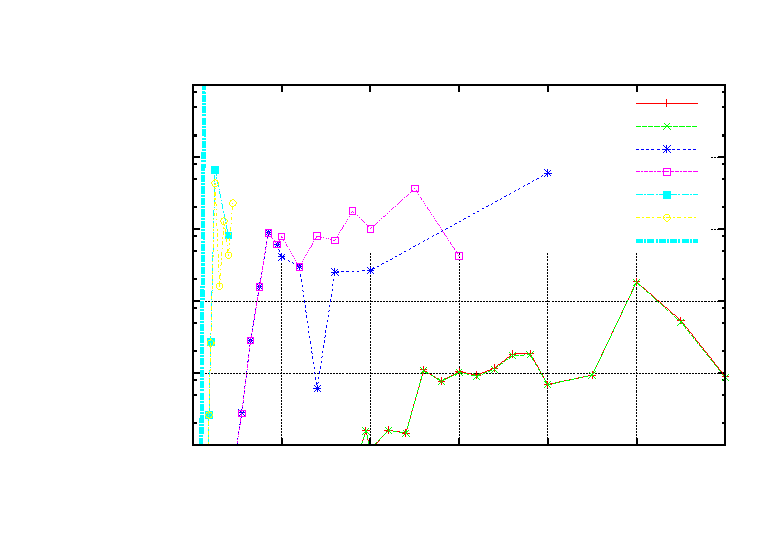
\includegraphics{ej2_nodos}}%
    \gplfronttext
  \end{picture}%
\endgroup
}
    \caption{Algoritmo exacto para grafos completos}
\end{figure}

\par Se puede observar en este gr\'afico, antes que nada, que la cota de complejidad
    se cumple efectivamente para las 3 familias de grafos seg\'un la densidad.

\par Tambi\'en se observa que para los grafos poco densos, no hay una diferencia
    notable entre las variantes del algoritmo (con la heur\'istica golosa o sin
    ella). Pero este patr\'on ya no se cumple si se observan las otras dos familias
    que nos quedan.

\par En el caso de la familia de los grafos \emph{regulares}, se destaca que a
    partir de los 500 nodos apr\'oximadamente, la variante que utiliza la cota
    derivada del \emph{N\'umero de Tur\'an}\footnote{Secci\'on~\ref{backtracking:poda:cota_front_min},
    \emph{\nameref{backtracking:poda:cota_front_min}}.} comienza a ser m\'as
    eficiente que la que utiliza la cota provista por la heur\'istica golosa.

\par Este comportamiento se invierte en el caso de las familias muy densas,
    observando como ya como mientras m\'as denso es el grafo, mejor es la cota
    de la heur\'istica que la cota te\'orica.

\bigskip

\par Por \'ultimo, analizamos los resultados para los grafos planares.

\begin{figure}[H]
    \centering
    \fontsize{8}{10}\selectfont
    \resizebox{1.0\textwidth}{!}{% GNUPLOT: LaTeX picture with Postscript
\begingroup
  \makeatletter
  \providecommand\color[2][]{%
    \GenericError{(gnuplot) \space\space\space\@spaces}{%
      Package color not loaded in conjunction with
      terminal option `colourtext'%
    }{See the gnuplot documentation for explanation.%
    }{Either use 'blacktext' in gnuplot or load the package
      color.sty in LaTeX.}%
    \renewcommand\color[2][]{}%
  }%
  \providecommand\includegraphics[2][]{%
    \GenericError{(gnuplot) \space\space\space\@spaces}{%
      Package graphicx or graphics not loaded%
    }{See the gnuplot documentation for explanation.%
    }{The gnuplot epslatex terminal needs graphicx.sty or graphics.sty.}%
    \renewcommand\includegraphics[2][]{}%
  }%
  \providecommand\rotatebox[2]{#2}%
  \@ifundefined{ifGPcolor}{%
    \newif\ifGPcolor
    \GPcolortrue
  }{}%
  \@ifundefined{ifGPblacktext}{%
    \newif\ifGPblacktext
    \GPblacktexttrue
  }{}%
  % define a \g@addto@macro without @ in the name:
  \let\gplgaddtomacro\g@addto@macro
  % define empty templates for all commands taking text:
  \gdef\gplbacktext{}%
  \gdef\gplfronttext{}%
  \makeatother
  \ifGPblacktext
    % no textcolor at all
    \def\colorrgb#1{}%
    \def\colorgray#1{}%
  \else
    % gray or color?
    \ifGPcolor
      \def\colorrgb#1{\color[rgb]{#1}}%
      \def\colorgray#1{\color[gray]{#1}}%
      \expandafter\def\csname LTw\endcsname{\color{white}}%
      \expandafter\def\csname LTb\endcsname{\color{black}}%
      \expandafter\def\csname LTa\endcsname{\color{black}}%
      \expandafter\def\csname LT0\endcsname{\color[rgb]{1,0,0}}%
      \expandafter\def\csname LT1\endcsname{\color[rgb]{0,1,0}}%
      \expandafter\def\csname LT2\endcsname{\color[rgb]{0,0,1}}%
      \expandafter\def\csname LT3\endcsname{\color[rgb]{1,0,1}}%
      \expandafter\def\csname LT4\endcsname{\color[rgb]{0,1,1}}%
      \expandafter\def\csname LT5\endcsname{\color[rgb]{1,1,0}}%
      \expandafter\def\csname LT6\endcsname{\color[rgb]{0,0,0}}%
      \expandafter\def\csname LT7\endcsname{\color[rgb]{1,0.3,0}}%
      \expandafter\def\csname LT8\endcsname{\color[rgb]{0.5,0.5,0.5}}%
    \else
      % gray
      \def\colorrgb#1{\color{black}}%
      \def\colorgray#1{\color[gray]{#1}}%
      \expandafter\def\csname LTw\endcsname{\color{white}}%
      \expandafter\def\csname LTb\endcsname{\color{black}}%
      \expandafter\def\csname LTa\endcsname{\color{black}}%
      \expandafter\def\csname LT0\endcsname{\color{black}}%
      \expandafter\def\csname LT1\endcsname{\color{black}}%
      \expandafter\def\csname LT2\endcsname{\color{black}}%
      \expandafter\def\csname LT3\endcsname{\color{black}}%
      \expandafter\def\csname LT4\endcsname{\color{black}}%
      \expandafter\def\csname LT5\endcsname{\color{black}}%
      \expandafter\def\csname LT6\endcsname{\color{black}}%
      \expandafter\def\csname LT7\endcsname{\color{black}}%
      \expandafter\def\csname LT8\endcsname{\color{black}}%
    \fi
  \fi
  \setlength{\unitlength}{0.0500bp}%
  \begin{picture}(7200.00,5040.00)%
    \gplgaddtomacro\gplbacktext{%
      \csname LTb\endcsname%
      \put(1034,924){\makebox(0,0)[r]{\strut{} 1}}%
      \csname LTb\endcsname%
      \put(1034,1270){\makebox(0,0)[r]{\strut{} 2}}%
      \csname LTb\endcsname%
      \put(1034,1615){\makebox(0,0)[r]{\strut{} 3}}%
      \csname LTb\endcsname%
      \put(1034,1961){\makebox(0,0)[r]{\strut{} 4}}%
      \csname LTb\endcsname%
      \put(1034,2306){\makebox(0,0)[r]{\strut{} 5}}%
      \csname LTb\endcsname%
      \put(1034,2652){\makebox(0,0)[r]{\strut{} 6}}%
      \csname LTb\endcsname%
      \put(1034,2997){\makebox(0,0)[r]{\strut{} 7}}%
      \csname LTb\endcsname%
      \put(1034,3343){\makebox(0,0)[r]{\strut{} 8}}%
      \csname LTb\endcsname%
      \put(1034,3688){\makebox(0,0)[r]{\strut{} 9}}%
      \csname LTb\endcsname%
      \put(1034,4034){\makebox(0,0)[r]{\strut{} 10}}%
      \csname LTb\endcsname%
      \put(1034,4379){\makebox(0,0)[r]{\strut{} 11}}%
      \csname LTb\endcsname%
      \put(1166,704){\makebox(0,0){\strut{} 0}}%
      \csname LTb\endcsname%
      \put(2106,704){\makebox(0,0){\strut{} 500}}%
      \csname LTb\endcsname%
      \put(3045,704){\makebox(0,0){\strut{} 1000}}%
      \csname LTb\endcsname%
      \put(3985,704){\makebox(0,0){\strut{} 1500}}%
      \csname LTb\endcsname%
      \put(4924,704){\makebox(0,0){\strut{} 2000}}%
      \csname LTb\endcsname%
      \put(5864,704){\makebox(0,0){\strut{} 2500}}%
      \csname LTb\endcsname%
      \put(6803,704){\makebox(0,0){\strut{} 3000}}%
      \put(176,2651){\rotatebox{-270}{\makebox(0,0){\strut{}Tiempo (microsegundos)}}}%
      \put(396,2651){\rotatebox{-270}{\makebox(0,0){\strut{}(Escala Lineal)}}}%
      \put(3984,374){\makebox(0,0){\strut{}Cantidad de Nodos}}%
      \put(3984,154){\makebox(0,0){\strut{}(Escala Lineal)}}%
      \put(3984,4709){\makebox(0,0){\strut{}Tiempo de ejecución conforme aumenta la cantidad de nodos}}%
    }%
    \gplgaddtomacro\gplfronttext{%
      \csname LTb\endcsname%
      \put(5816,1537){\makebox(0,0)[r]{\strut{}Planar }}%
      \csname LTb\endcsname%
      \put(5816,1317){\makebox(0,0)[r]{\strut{}Planar (Golosa)}}%
      \csname LTb\endcsname%
      \put(5816,1097){\makebox(0,0)[r]{\strut{}Cota teórica superior $\mathcal O(n^5)$}}%
    }%
    \gplbacktext
    \put(0,0){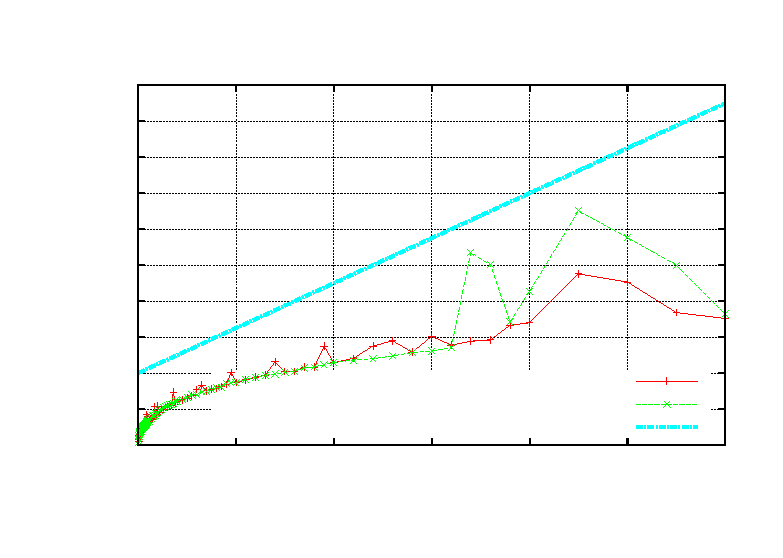
\includegraphics{ej2_nodos_planar}}%
    \gplfronttext
  \end{picture}%
\endgroup
}
    \caption{Algoritmo exacto para grafos planares}
\end{figure}

\par A la hora de realizar este gr\'afico, decidimos tomar los datos experimentales
    y tomarles la ra\'iz quinta, ya que al tener una conta te\'orica
    $\mathcal O(n^5)$, haciendo esto estamos "linealizando" las medidas, haciendo
    m\'as f\'acil la comparaci\'on experimental para comprobar que la cota te\'orica
    hayada efectivamente se cumple.

\par Como se puede ver en el gr\'afico, estos datos linealizados est\'an acotados
    por una funci\'on lineal (que, dada la linealizaci\'on, pasa a representar a
    la cota te\'orica $\mathcal O(n^5)$.), cumpli\'endose entonces la cota an\'alizada
    para esta familia.

\bigskip

\par A continuaci\'on se exhiben dos gr\'aficos, donde cambiamos el eje observacional
    de la complejidad: en lugar de ver la relaci\'on entre el tiempo de ejecuci\'on
    necesario para resolver un problema en funci\'on de los nodos, lo planteamos en
    funci\'on de la cantidad de ejes.

\begin{figure}[H]
    \centering
    \fontsize{8}{10}\selectfont
    \resizebox{1.0\textwidth}{!}{% GNUPLOT: LaTeX picture with Postscript
\begingroup
  \makeatletter
  \providecommand\color[2][]{%
    \GenericError{(gnuplot) \space\space\space\@spaces}{%
      Package color not loaded in conjunction with
      terminal option `colourtext'%
    }{See the gnuplot documentation for explanation.%
    }{Either use 'blacktext' in gnuplot or load the package
      color.sty in LaTeX.}%
    \renewcommand\color[2][]{}%
  }%
  \providecommand\includegraphics[2][]{%
    \GenericError{(gnuplot) \space\space\space\@spaces}{%
      Package graphicx or graphics not loaded%
    }{See the gnuplot documentation for explanation.%
    }{The gnuplot epslatex terminal needs graphicx.sty or graphics.sty.}%
    \renewcommand\includegraphics[2][]{}%
  }%
  \providecommand\rotatebox[2]{#2}%
  \@ifundefined{ifGPcolor}{%
    \newif\ifGPcolor
    \GPcolortrue
  }{}%
  \@ifundefined{ifGPblacktext}{%
    \newif\ifGPblacktext
    \GPblacktexttrue
  }{}%
  % define a \g@addto@macro without @ in the name:
  \let\gplgaddtomacro\g@addto@macro
  % define empty templates for all commands taking text:
  \gdef\gplbacktext{}%
  \gdef\gplfronttext{}%
  \makeatother
  \ifGPblacktext
    % no textcolor at all
    \def\colorrgb#1{}%
    \def\colorgray#1{}%
  \else
    % gray or color?
    \ifGPcolor
      \def\colorrgb#1{\color[rgb]{#1}}%
      \def\colorgray#1{\color[gray]{#1}}%
      \expandafter\def\csname LTw\endcsname{\color{white}}%
      \expandafter\def\csname LTb\endcsname{\color{black}}%
      \expandafter\def\csname LTa\endcsname{\color{black}}%
      \expandafter\def\csname LT0\endcsname{\color[rgb]{1,0,0}}%
      \expandafter\def\csname LT1\endcsname{\color[rgb]{0,1,0}}%
      \expandafter\def\csname LT2\endcsname{\color[rgb]{0,0,1}}%
      \expandafter\def\csname LT3\endcsname{\color[rgb]{1,0,1}}%
      \expandafter\def\csname LT4\endcsname{\color[rgb]{0,1,1}}%
      \expandafter\def\csname LT5\endcsname{\color[rgb]{1,1,0}}%
      \expandafter\def\csname LT6\endcsname{\color[rgb]{0,0,0}}%
      \expandafter\def\csname LT7\endcsname{\color[rgb]{1,0.3,0}}%
      \expandafter\def\csname LT8\endcsname{\color[rgb]{0.5,0.5,0.5}}%
    \else
      % gray
      \def\colorrgb#1{\color{black}}%
      \def\colorgray#1{\color[gray]{#1}}%
      \expandafter\def\csname LTw\endcsname{\color{white}}%
      \expandafter\def\csname LTb\endcsname{\color{black}}%
      \expandafter\def\csname LTa\endcsname{\color{black}}%
      \expandafter\def\csname LT0\endcsname{\color{black}}%
      \expandafter\def\csname LT1\endcsname{\color{black}}%
      \expandafter\def\csname LT2\endcsname{\color{black}}%
      \expandafter\def\csname LT3\endcsname{\color{black}}%
      \expandafter\def\csname LT4\endcsname{\color{black}}%
      \expandafter\def\csname LT5\endcsname{\color{black}}%
      \expandafter\def\csname LT6\endcsname{\color{black}}%
      \expandafter\def\csname LT7\endcsname{\color{black}}%
      \expandafter\def\csname LT8\endcsname{\color{black}}%
    \fi
  \fi
  \setlength{\unitlength}{0.0500bp}%
  \begin{picture}(7200.00,5040.00)%
    \gplgaddtomacro\gplbacktext{%
      \csname LTb\endcsname%
      \put(1562,924){\makebox(0,0)[r]{\strut{} 0.001}}%
      \csname LTb\endcsname%
      \put(1562,1270){\makebox(0,0)[r]{\strut{} 0.01}}%
      \csname LTb\endcsname%
      \put(1562,1615){\makebox(0,0)[r]{\strut{} 0.1}}%
      \csname LTb\endcsname%
      \put(1562,1961){\makebox(0,0)[r]{\strut{} 1}}%
      \csname LTb\endcsname%
      \put(1562,2306){\makebox(0,0)[r]{\strut{} 10}}%
      \csname LTb\endcsname%
      \put(1562,2652){\makebox(0,0)[r]{\strut{} 100}}%
      \csname LTb\endcsname%
      \put(1562,2997){\makebox(0,0)[r]{\strut{} 1000}}%
      \csname LTb\endcsname%
      \put(1562,3343){\makebox(0,0)[r]{\strut{} 10000}}%
      \csname LTb\endcsname%
      \put(1562,3688){\makebox(0,0)[r]{\strut{} 100000}}%
      \csname LTb\endcsname%
      \put(1562,4034){\makebox(0,0)[r]{\strut{} 1e+06}}%
      \csname LTb\endcsname%
      \put(1562,4379){\makebox(0,0)[r]{\strut{} 1e+07}}%
      \csname LTb\endcsname%
      \put(1694,704){\makebox(0,0){\strut{} 1}}%
      \csname LTb\endcsname%
      \put(2424,704){\makebox(0,0){\strut{} 10}}%
      \csname LTb\endcsname%
      \put(3154,704){\makebox(0,0){\strut{} 100}}%
      \csname LTb\endcsname%
      \put(3884,704){\makebox(0,0){\strut{} 1000}}%
      \csname LTb\endcsname%
      \put(4613,704){\makebox(0,0){\strut{} 10000}}%
      \csname LTb\endcsname%
      \put(5343,704){\makebox(0,0){\strut{} 100000}}%
      \csname LTb\endcsname%
      \put(6073,704){\makebox(0,0){\strut{} 1e+06}}%
      \csname LTb\endcsname%
      \put(6803,704){\makebox(0,0){\strut{} 1e+07}}%
      \put(176,2651){\rotatebox{-270}{\makebox(0,0){\strut{}Tiempo (milisegundos)}}}%
      \put(396,2651){\rotatebox{-270}{\makebox(0,0){\strut{}(Escala Logaritmica)}}}%
      \put(4248,374){\makebox(0,0){\strut{}Cantidad de ejes}}%
      \put(4248,154){\makebox(0,0){\strut{}(Escala Logaritmica)}}%
      \put(4248,4709){\makebox(0,0){\strut{}Tiempo de ejecución conforme aumenta la cantidad de ejes}}%
    }%
    \gplgaddtomacro\gplfronttext{%
      \csname LTb\endcsname%
      \put(5816,1537){\makebox(0,0)[r]{\strut{}Poco denso}}%
      \csname LTb\endcsname%
      \put(5816,1317){\makebox(0,0)[r]{\strut{}Regular}}%
      \csname LTb\endcsname%
      \put(5816,1097){\makebox(0,0)[r]{\strut{}Denso}}%
    }%
    \gplbacktext
    \put(0,0){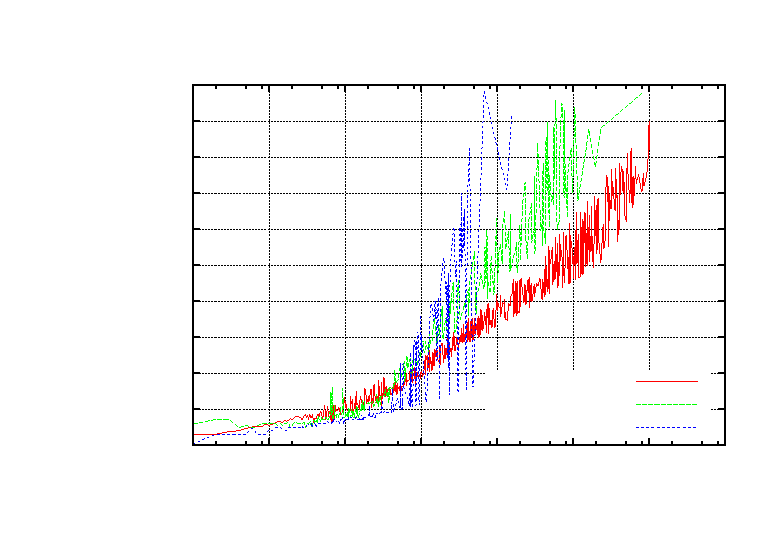
\includegraphics{ej2_ejes}}%
    \gplfronttext
  \end{picture}%
\endgroup
}
    \caption{Algoritmo exacto en funci\'on de los ejes}
\end{figure}

\par En este gr\'afico se puede observar como el comportamiento de la complejidad
    es bastante m\'as, si se quiere, constante. Si bien vemos un comportamiento
    de picos irregular (debido a las podas implementadas, que no siempre tendr\'an
    el mismo efecto en todos los grafos), el incremento promedio que se puede
    observar marca como el crecimiento para densos (es decir, muchas aristas para
    una cantidad fija de nodos) supera ampliamente a aquellos grafos menos densos.

\par Es decir, podemos observar que a igual cantidad de nodos, aquellos grafos
    m\'as densos requieren mayor tiempo para ser procesados.

\begin{figure}[H]
    \centering
    \fontsize{8}{10}\selectfont
    \resizebox{1.0\textwidth}{!}{% GNUPLOT: LaTeX picture with Postscript
\begingroup
  \makeatletter
  \providecommand\color[2][]{%
    \GenericError{(gnuplot) \space\space\space\@spaces}{%
      Package color not loaded in conjunction with
      terminal option `colourtext'%
    }{See the gnuplot documentation for explanation.%
    }{Either use 'blacktext' in gnuplot or load the package
      color.sty in LaTeX.}%
    \renewcommand\color[2][]{}%
  }%
  \providecommand\includegraphics[2][]{%
    \GenericError{(gnuplot) \space\space\space\@spaces}{%
      Package graphicx or graphics not loaded%
    }{See the gnuplot documentation for explanation.%
    }{The gnuplot epslatex terminal needs graphicx.sty or graphics.sty.}%
    \renewcommand\includegraphics[2][]{}%
  }%
  \providecommand\rotatebox[2]{#2}%
  \@ifundefined{ifGPcolor}{%
    \newif\ifGPcolor
    \GPcolortrue
  }{}%
  \@ifundefined{ifGPblacktext}{%
    \newif\ifGPblacktext
    \GPblacktexttrue
  }{}%
  % define a \g@addto@macro without @ in the name:
  \let\gplgaddtomacro\g@addto@macro
  % define empty templates for all commands taking text:
  \gdef\gplbacktext{}%
  \gdef\gplfronttext{}%
  \makeatother
  \ifGPblacktext
    % no textcolor at all
    \def\colorrgb#1{}%
    \def\colorgray#1{}%
  \else
    % gray or color?
    \ifGPcolor
      \def\colorrgb#1{\color[rgb]{#1}}%
      \def\colorgray#1{\color[gray]{#1}}%
      \expandafter\def\csname LTw\endcsname{\color{white}}%
      \expandafter\def\csname LTb\endcsname{\color{black}}%
      \expandafter\def\csname LTa\endcsname{\color{black}}%
      \expandafter\def\csname LT0\endcsname{\color[rgb]{1,0,0}}%
      \expandafter\def\csname LT1\endcsname{\color[rgb]{0,1,0}}%
      \expandafter\def\csname LT2\endcsname{\color[rgb]{0,0,1}}%
      \expandafter\def\csname LT3\endcsname{\color[rgb]{1,0,1}}%
      \expandafter\def\csname LT4\endcsname{\color[rgb]{0,1,1}}%
      \expandafter\def\csname LT5\endcsname{\color[rgb]{1,1,0}}%
      \expandafter\def\csname LT6\endcsname{\color[rgb]{0,0,0}}%
      \expandafter\def\csname LT7\endcsname{\color[rgb]{1,0.3,0}}%
      \expandafter\def\csname LT8\endcsname{\color[rgb]{0.5,0.5,0.5}}%
    \else
      % gray
      \def\colorrgb#1{\color{black}}%
      \def\colorgray#1{\color[gray]{#1}}%
      \expandafter\def\csname LTw\endcsname{\color{white}}%
      \expandafter\def\csname LTb\endcsname{\color{black}}%
      \expandafter\def\csname LTa\endcsname{\color{black}}%
      \expandafter\def\csname LT0\endcsname{\color{black}}%
      \expandafter\def\csname LT1\endcsname{\color{black}}%
      \expandafter\def\csname LT2\endcsname{\color{black}}%
      \expandafter\def\csname LT3\endcsname{\color{black}}%
      \expandafter\def\csname LT4\endcsname{\color{black}}%
      \expandafter\def\csname LT5\endcsname{\color{black}}%
      \expandafter\def\csname LT6\endcsname{\color{black}}%
      \expandafter\def\csname LT7\endcsname{\color{black}}%
      \expandafter\def\csname LT8\endcsname{\color{black}}%
    \fi
  \fi
  \setlength{\unitlength}{0.0500bp}%
  \begin{picture}(7200.00,5040.00)%
    \gplgaddtomacro\gplbacktext{%
      \csname LTb\endcsname%
      \put(1562,924){\makebox(0,0)[r]{\strut{} 0.0001}}%
      \csname LTb\endcsname%
      \put(1562,1500){\makebox(0,0)[r]{\strut{} 0.01}}%
      \csname LTb\endcsname%
      \put(1562,2076){\makebox(0,0)[r]{\strut{} 1}}%
      \csname LTb\endcsname%
      \put(1562,2652){\makebox(0,0)[r]{\strut{} 100}}%
      \csname LTb\endcsname%
      \put(1562,3227){\makebox(0,0)[r]{\strut{} 10000}}%
      \csname LTb\endcsname%
      \put(1562,3803){\makebox(0,0)[r]{\strut{} 1e+06}}%
      \csname LTb\endcsname%
      \put(1562,4379){\makebox(0,0)[r]{\strut{} 1e+08}}%
      \csname LTb\endcsname%
      \put(1694,704){\makebox(0,0){\strut{} 1}}%
      \csname LTb\endcsname%
      \put(2424,704){\makebox(0,0){\strut{} 10}}%
      \csname LTb\endcsname%
      \put(3154,704){\makebox(0,0){\strut{} 100}}%
      \csname LTb\endcsname%
      \put(3884,704){\makebox(0,0){\strut{} 1000}}%
      \csname LTb\endcsname%
      \put(4613,704){\makebox(0,0){\strut{} 10000}}%
      \csname LTb\endcsname%
      \put(5343,704){\makebox(0,0){\strut{} 100000}}%
      \csname LTb\endcsname%
      \put(6073,704){\makebox(0,0){\strut{} 1e+06}}%
      \csname LTb\endcsname%
      \put(6803,704){\makebox(0,0){\strut{} 1e+07}}%
      \put(176,2651){\rotatebox{-270}{\makebox(0,0){\strut{}Tiempo (milisegundos)}}}%
      \put(396,2651){\rotatebox{-270}{\makebox(0,0){\strut{}(Escala Logaritmica)}}}%
      \put(4248,374){\makebox(0,0){\strut{}Cantidad de ejes}}%
      \put(4248,154){\makebox(0,0){\strut{}(Escala Logaritmica)}}%
      \put(4248,4709){\makebox(0,0){\strut{}Tiempo de ejecución conforme aumenta la cantidad de ejes}}%
    }%
    \gplgaddtomacro\gplfronttext{%
      \csname LTb\endcsname%
      \put(5816,1537){\makebox(0,0)[r]{\strut{}Poco denso (Golosa)}}%
      \csname LTb\endcsname%
      \put(5816,1317){\makebox(0,0)[r]{\strut{}Regular (Golosa)}}%
      \csname LTb\endcsname%
      \put(5816,1097){\makebox(0,0)[r]{\strut{}Denso (Golosa)}}%
    }%
    \gplbacktext
    \put(0,0){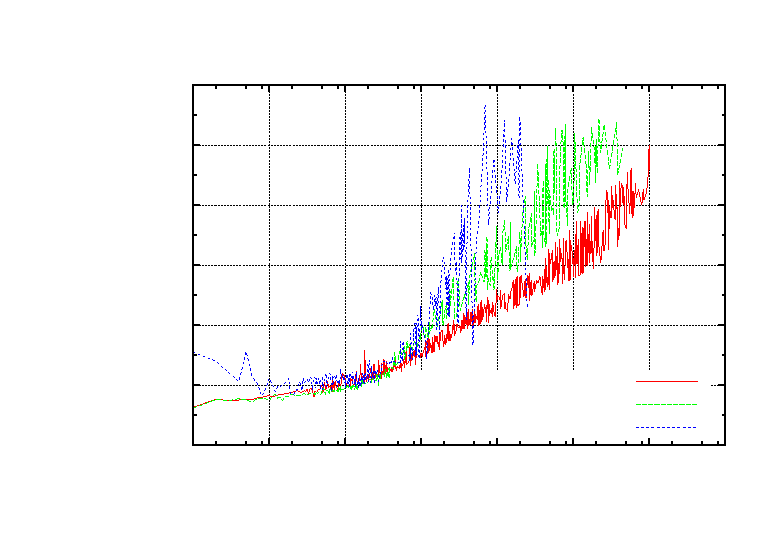
\includegraphics{ej2_ejes_golosa}}%
    \gplfronttext
  \end{picture}%
\endgroup
}
    \caption{Algoritmo exacto en funci\'on de los ejes (variante golosa)}
\end{figure}

\par En este segundo gr\'afico, podemos observar que el comportamiento detallado
    para el algoritmo que utiliza la cota de frontera m\'inima te\'orica se
    mantiene (e incluso, se ve a\'un m\'as marcado) para la variante que utiliza
    el resultado de la heur\'istica golosa.

\subsubsection{Conclusiones}
\par De la experimentaci\'on realizada podemos observar que el principal par\'ametro
    que afecta al tiempo de corrida de nuestro algoritmo es la relaci\'on entre
    los nodos y la cantidad de aristas del grafo de entrada.

\par Si bien, sin importar si el grafo es denso o no, a medida que este vaya
    incrementando su tama\~no en nodos y/o aristas, la complejidad del algoritmo
    seguir\'a incrementandose asint\'oticamente. Pero por motivos didactos,
    es interesante observar como el crecimiento de la complejidad se ve
    m\'as relacionada con la densidad del grafo (a igual cantidad de nodos, grafos
    m\'as densos toman m\'as tiempo).

\par Tambi\'en es interesante deducir que para grafos poco densos (como los planares),
    el algoritmo exacto se comporta muy bien con una complejidad (en la realidad),
    tendiendo a polinomial (para los planares esto ha quedado demostrado). M\'as
    detalles sobre esta conclusi\'on se exhiben en la Secci\'on~\ref{experimentacion}
    (\emph{\nameref{experimentacion}}).

\par A su vez, tambi\'en pudimos comprobar el resultado te\'orico explayado
    en~\nameref{backtracking:poda:grafo_completo}, mediante el cual comprobamos
    en caso de ser el grafo de entrada un grafo completo, la soluci\'on exacta
    se computa en tiempo lineal en la cantidad de nodos.
